\chapter{背景介绍}
\label{cha:intro}

在介绍卷积神经网络(Convolutional Neural Network,简称为  CNN)的相关理论结果之前,我们先对卷积神经网络的发展,卷积神经网络的应用成果以及卷积神经网络的工作方式进行一定的介绍。

\section{卷积神经网络的发展历史}
对于CNN的提出有重大影响的工作最早可以追溯到1968年Hubel和Wiesel的一次对猫的视觉反应的观察实验。他们将示波器连接到猫的视觉神经上,观察猫在看到不同图像时,示波器的波形的变化。他们的实验发现视觉的处理过程中,部分输入信息被丢失,多个输入对应到了同一个输出,也就是说,部分信息被神经元“过滤”了。因为这项工作Hubel和Wiesel共享了1981年诺贝尔奖。而在1980年,日本科学家Kunihiko Fukishima(福岛邦彦)受到Hubel和Wiesel实验的启发,发表了题为《Neocognitron: A self-organizing neural network model for a mechanism of pattern recognition unaffected by shift in position》的论文\cite{fukushima1980neocognitron},提出了Neocongnitron。这篇工作中,Kunihiko Fukishima在人工神经网络中引入了人类视觉系统的概念,提出了现在成为卷积和池化的概念,普遍认为这是现在CNN的雏形。
\par
在之后的大约十年内,虽然有很多研究者基于Kunihiko Fukishima的Neocognitron提出了一些模型,但是都没有大的突破,直到1989年,Yann LeCun在《Backpropagation applied to handwritten zip code recognition》 \cite{lecun1989backpropagation}中吸取了Neocognitron的核心思想,并且引入了LeCun在Back Propogation方面的工作。在这篇论文中LeCun定义了新的卷积操作,使得网络的泛化能力提高,训练速度也加快。
\par
1998年,\citet{lecun1998gradient}提出了LeNet-5,这时的LeNet-5与现在的CNN的结构基本一致,只是在最后一层输出层,LeNet-5没有使用Fully Connected Layer,而是RBF Layer。LeNet-5的出现使得CNN的使用出现了一次高潮,但是由于计算能力的限制,与现在的应用水平相比还相去甚远。
\par
2006年,\citet{bouvrie2006notes}给出了CNN的推导和实现公式,而在之后的几年内,关于CNN的工作没有较大的突破。直到2012年,深度学习三巨头之一的Geoffrey Hinton的团队提出了基于CNN的深度神经网络AlexNet。AlexNet在ImageNet LSVRC-2012分类任务上以压倒性优势获得了最高的准确率。AlexNet的出现使得人们认识到了CNN在图像任务上的优势,在之后的几年里,不断有基于CNN的神经网络被提出,例如2013年提出的VGG\cite{simonyan2014very}和2014年提出的GoogleNet\cite{szegedy2015going},他们在ImageNet LSVRC上的表现都已经远超AlexNet,但是首次实现神经网络的识别准确率高于人类的模型是2016年\citet{he2016deep}提出的ResNet。ResNet将神经网络的深度提高了一个数量级,大大加快了神经网络的训练速度,并且提高了神经网络的识别准确率。在这之前还有很多基于CNN的网络被研究者提出,但是他们的贡献不是很突出,例如Fast RCNN\cite{girshick2015fast},SPP Net\cite{he2015spatial}等。
\begin{figure}
\centering
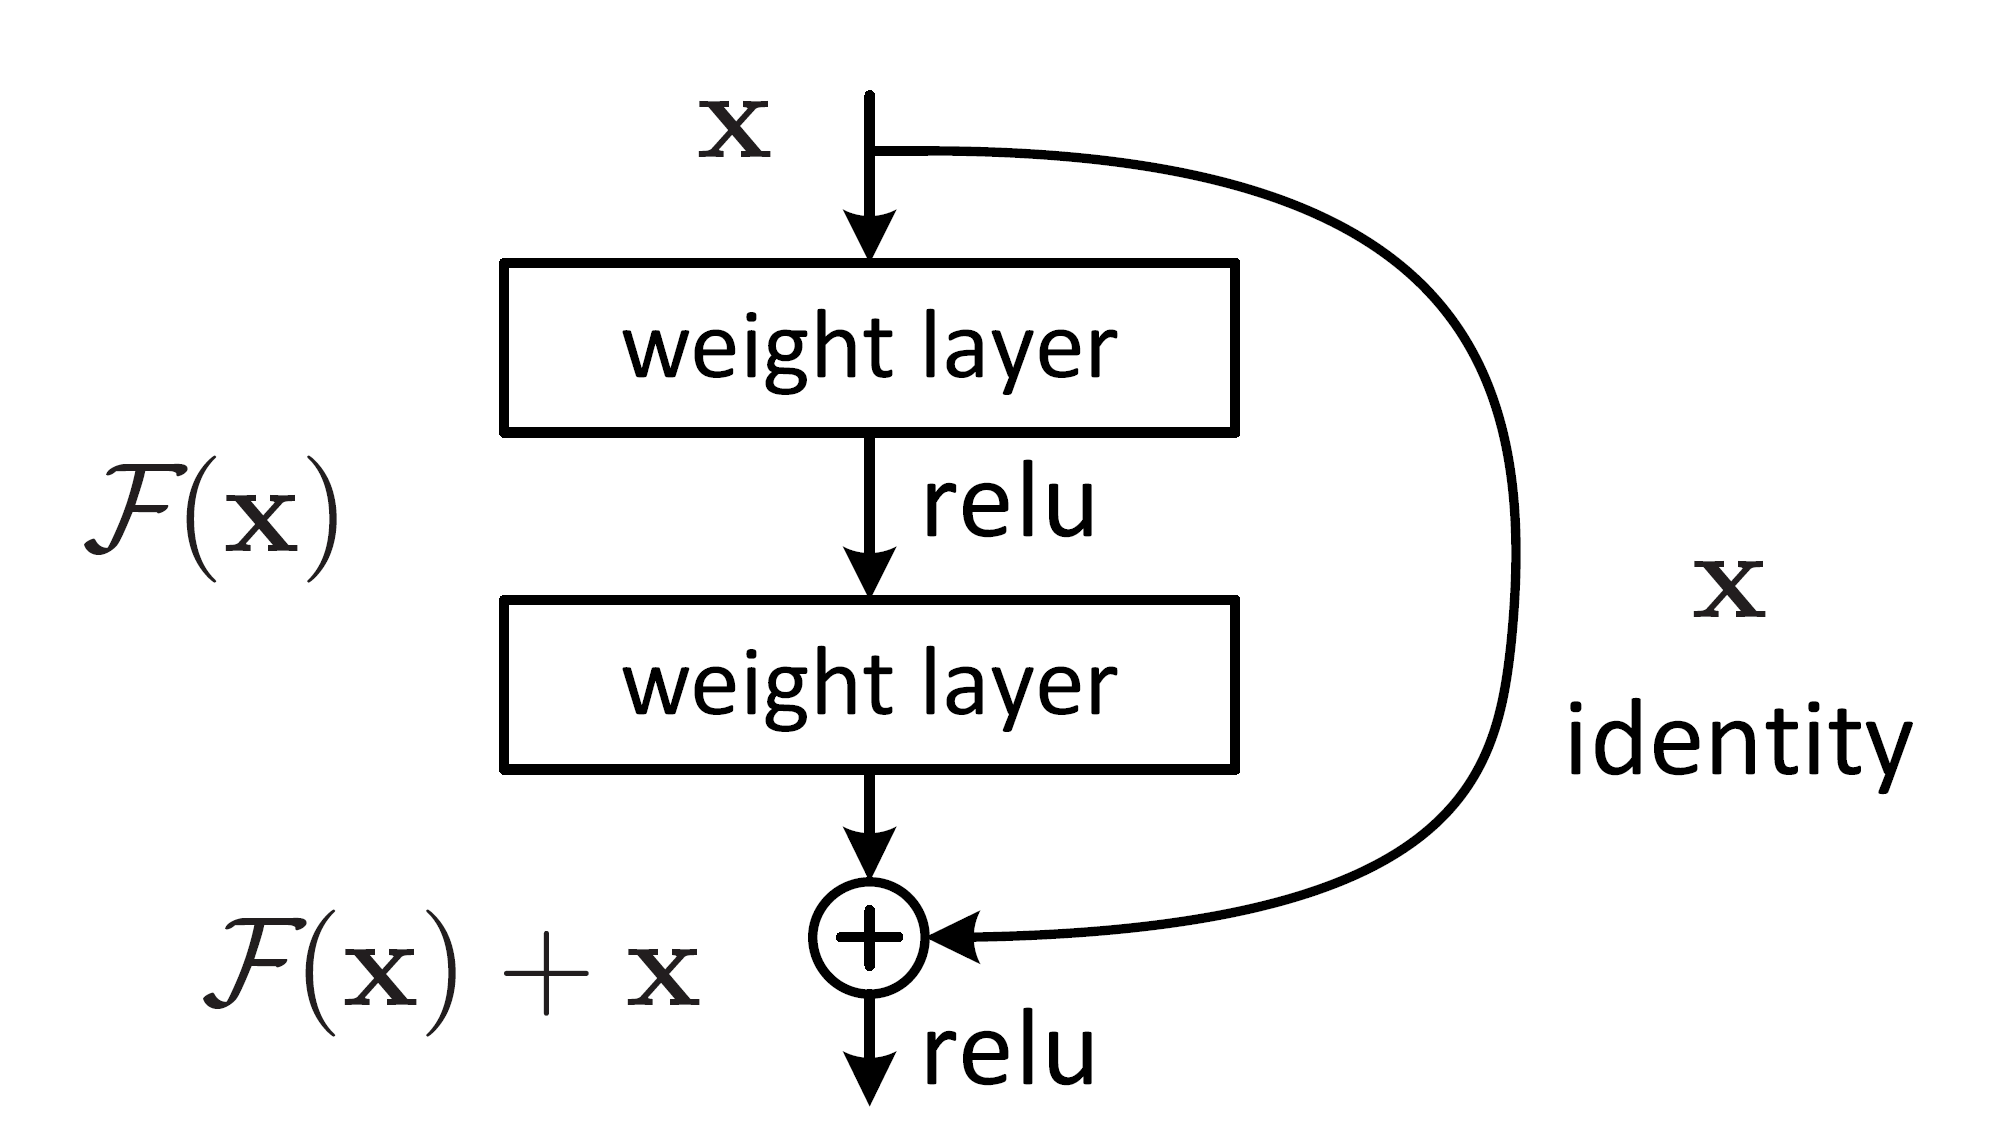
\includegraphics[width=10cm]{./figures/ResNet.PNG}
\caption{ResNet的结构\cite{he2016deep}}
\label{fig:Res}
\end{figure}


\section{卷积神经网络的工作过程}
卷积神经网络一般由卷积层,池化层,全连接层,激活层组成。简要的说,卷积层是将输入的数据信息进行过滤,池化层是对输入数据进行压缩,激活函数则是为了引入非线性而加入网络中的函数,全连接层往往用在最后一层,将卷积和池化后的数据对应到输出。下面,本文将详细的说明卷积神经网络层和池化层在处理图像数据时的作用。
\begin{itemize}
  \item 卷积层:卷积层是通过一个滤波器(卷积核),将滤波器覆盖输入的数据,并进行窗口移动,每次都与覆盖的数据进行元素间的相乘,并将相乘结果相加除以元素个数得到该窗口对应的输出值。具体说来,假设输入数据为$x\in \mathbb{R}^{n\times n}$, 滤波器为$f\in \mathbb{R}^{l\times l}$, 则输出$y\in \mathbb{R}^{(n-l+1)\times (n-l+1)}$,其中
  \[
    y_{i,j} = \frac{1}{l^2}\sum_{s = j}^{j+l-1}\sum_{t = i}^{i+l-1} x_{t,s}f_{t-i+1,s-i+1}.
  \]
  \par
  图~\ref{fig:conv}~是上述过程的一个直观的说明图。
  \begin{figure}
  \centering
  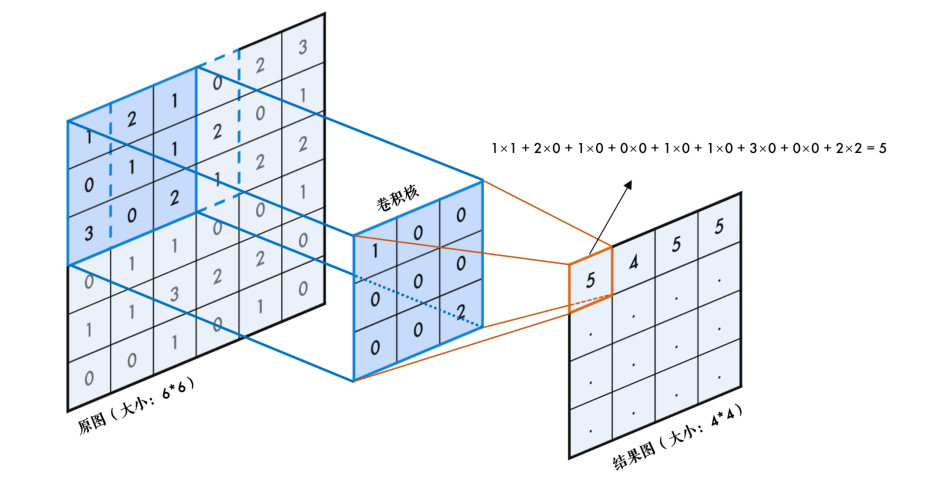
\includegraphics[width=10cm]{./figures/conv.jpg}
  \caption{卷积层工作原理示意}
  \label{fig:conv}
  \end{figure}
  \par
  卷积实际上就是计算卷积核与窗口数据之间的相似程度,但是当卷积核窗口移动时,相邻窗口之间有很多部分是重叠的,这就意味着最后的输出中有大量的重复的信息,这样的重复信息大大增加了计算的难度并且降低了计算效率。而这些重复的信息,实际上并不是需要的,神经网络需要一种机制对重复信息进行舍弃,这就是池化层的功能。
  \item 池化层:	池化层有很多种,这里我们以平均池化为例进行介绍。假设池化层的输入为$x\in \mathbb{R}^{m\times m}$,池化窗口为$d\times d$,为了简单起见,进一步假设$m\equiv 0 (\mod d)$,这个假设只是为了叙述方便,不会对结果有本质影响。
  \par
  池化层的输出为$y\in \mathbb{R}^{k\times k}$,其中$k = m/d$,且
  \[
  	y_{i,j} = \frac{1}{d^2}\sum_{s=(i-1)d+1}^{id}\sum_{t=(j-1)d+1}^{jd}x_{s,t}.
  \]
  \par
  图~\ref{fig:avgpool}~展示了以$2\times2$为单位进行平均池化的一个实例。
  \begin{figure}
  \centering
  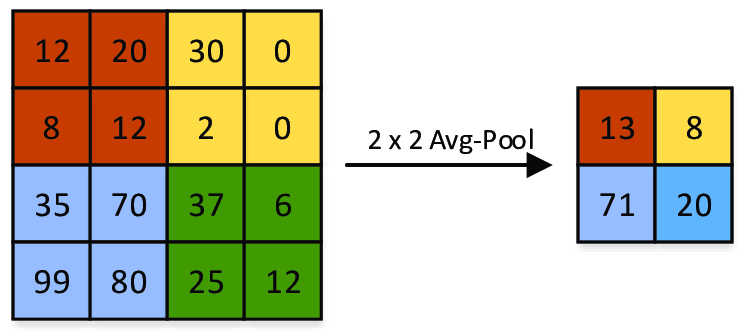
\includegraphics[width=10cm]{./figures/avgpool.png}
  \caption{平均池化的实例}
  \label{fig:avgpool}
  \end{figure}
  \par
  池化层的重要意义在于,它可以将数据进行降维,图像数据往往维度都很大,计算量很大,而进行降维可以大大降低计算量。另一方面,由于池化具有平移不变性,当输入数据受到微小扰动时,池化层的输出也会保持不变,神经网络的鲁棒性(Robustness)增强了。
\end{itemize}



\section{本文主要记号}
这一部分我们将简要介绍本文使用到的主要记号及其含义。
\par
我们用$x_i$表示输入的第$i$个数据,$X = (x_i)_i$表示组成的矩阵,$y_i$表示$x_i$对应的输入值/标签,$n$表示输入数据的个数,$\mathcal{D}$表示输入数据服从的概率分布。我们用$w,a$表示网络中的权重参数,$m$表示网络的宽度,$f(\cdot)$表示模型的预测值,$l(\cdot)$表示损失函数,$L$表示网络的层数,$\eta$表示学习率。$\mathbb{I}$表示示性函数,$\mathbb{E}$是数学期望的符号,$\mathbb{P}$和$P$表示概率测度,$\sigma(\cdot)$表示激活函数,$\|\cdot\|$表示范数,$\mathcal{N}(\mu,\Sigma^\top \Sigma)$表示均值为$\mu$,方差为$\Sigma^\top\Sigma$的正态分布。我们用$O(\cdot),\Theta(\cdot)$和$\Omega(\cdot)$分别表示最差、近似和最好的复杂度情况,$\tilde{O}$表示舍去复杂度中的$\log$项后的复杂度。我们用$\lesssim$表示舍去常数下的$<$。$[n]$表示$\{1,2,\cdots,n\}$,$poly(\cdot)$表示多项式函数。